\chapter{Diseño e implementación}
\label{cap:diseñoeimplementación}

%Hacer intro de esta sección, supongo que cuando esté algo más hecho será más fácil hacerla.

Hemos planteado la aplicación como un modelo cliente-servidor, en la que el servidor se encargará de ejecutar el programa que lleve a cabo todos los cálculos y se los proporcionará al cliente (dispositivo móvil) cuando este lo solicite. De esta manera, nuestro programa estará mejor organizado, será mas rápido y evitaremos que nuestro dispositivo móvil se quede sin batería en el cálculo de datos. A continuación detallaremos el diseño y la implementación tanto del cliente como del servidor.


\section{Servidor}
El servidor es una parte indispensable del proyecto ya que se encarga de realizar los cálculos más pesados para no sobrecargar al dispositivo móvil. Las principales tareas de las que se encarga son:
\begin{itemize}
	\item Permanecer a la escucha de cualquier cliente que solicite conexión.
	\item Solventar el posicionamiento del cliente conectado.
	\item Generar la mejor ruta (más corta y mejor adaptada) desde la posición actual hasta el destino indicado.
	\item Enviar la siguiente instruacción al cliente.	
\end{itemize} 

La aplicación servidor se divide en código java y los archivos .xml en los que se encuentra la información del edificio. Buena parte del código que los conforma ha sido reutilizado de trabajos anteriores, en concreto del proyecto BLABLABLA \cite{TFGguia} y del de MARIANA. Sin embargo se han introducido cambios notorios para el desarrollo de esta aplicación que comentaremos a continuación.
\subsection{Archivos XML}
-completar
\subsection{Código java}
Para entender mejor la estructura de nuestro servidor, veamos las principales clases de las que se compone y su función (en la \ref{fig:diagServ} se puede ver el diagrama con las dependencias de cada una de ellas):

\begin{itemize}
	\item \textit{MainClienteAndroid}: como su propio nombre indica, es el \textit{Main} del servidor. Se hizo otra versión para probar el servidor sin necesidad de acceder a el mediante la aplicación móvil, es por ello que lleva el identificador de Ciente Android en el nombre. Esta clase se encarga de la conexión directa con el cliente, abre un \textit{ServerSocket} que queda a la espera de clientes y, una vez llegan, los atiende. Es decir, lee sus posiciones origen y destino al que se quieren dirigir y devuelve la siguiente instrucción que deben seguir, para lo cual se apoya en distintas clases que detallamos a continuación. 
	
	\item \textit{Edificio}: esta clase es muy importante, pues guarda la información relativa al mapeo: los cuadrantes y las estancias. En nuestro caso, estas últimas se corresponden con las plantas del edificio, para la Facultad de Informática tenemos dos estancias, la planta baja y la primera planta. \textit{Edificio} se apoya en \textit{CargaXML}, cuya misión es leer toda la información que se recoge en los archivos xml que hemos visto con anterioridad.
	
	\item \textit{Estancia} y \textit{Cuadrante}: su propio nombre es muy descriptivo. \textit{Estancia} guarda la información de los cuadrantes que hay en cada planta y tiene funciones que permiten saber si un cuadrante está en una determinada estancia o añadir un cuadrante a una estancia, por ejemplo. En el caso de la clase \textit{Cuadrante} tenemos estructuras que guardan toda la información referente al cuadrante, como son su identificador, el \textit{beacon} que le corresponde, la información que tiene asociada, los metros que ocupa, la planta en la que está y, una de las cosas más importantes, con quién está conectado. 
	
	\item \textit{ListaCuadrantes}: esta clase constituye una parte importante, pues es la encargada de formar la matriz de adyacencia a partir de la información de conexión de cada cuadrante. Es aquí donde introducimos los pesos que tendrá cada conexión en función de la dificultad de la misma para una persona con discapacidad visual. Veremos esto con más detalle en la Sección \ref{rutaEInst}. Además, es la encargada de obtener la lista de cuadrantes que conformarán la ruta del origen al destino mediante el algoritmo de \textit{Dijkstra}.
	
	\item \textit{GerenarRuta}: llegamos ahora a la clase estrella, la encargada de la generación de las instrucciones que debe seguir el cliente. En la función \textit{genera} se guarda la lógica referente a ello. Es la función que más modificaciones a sufrido con respecto a los trabajos previos, pues debíamos adaptar las instrucciones a personas con discapacidad visual. Eso implicaba dar instrucciones mucho más precisas e informadas. Por ejemplo, en lugar de finalizar la ruta con \textit{ha llegado a su destino} ahora se indica dónde está el destino, dependiendo de la ruta que se haya seguido. Podría ser: \textit{su destino está a la derecha}. Ahora en la ruta también se incluye información anticipada sobre lo que el usuario se va a encontrar, como pueden ser pequeños escalones, baños o el despacho de Delegación de Alumnos. Esto es fundamental, pues da seguridad al usuario, si sabe lo que va a venir puede prepararse y actuar en consecuencia. Otra ampliación que se ha introducido es la del cambio de planta. En los trabajos anteriores no se contemplaba pero ahora la planta baja y la primera planta están unidas por los cuadrantes correspondientes a los ascensores, permitiendo así tener origen y destino en plantas distintas. A pesar de que en la Facultad de Informática contamos con ascensores y escaleras, se ha supuesto que la ruta se seguirá por medio de los ascensores, pues es más fácil el cambio de planta y, además, están adaptados con \textit{braille}.
	
	\item \textit{Persona}: esta clase guarda la información referente a la información del cliente, principalmente el origen y el destino de la ruta que quiere hacer y la propia ruta, es decir, la lista de cuadrantes que hay que seguir.
\end{itemize}


\begin{figure}[t]
	\centering
	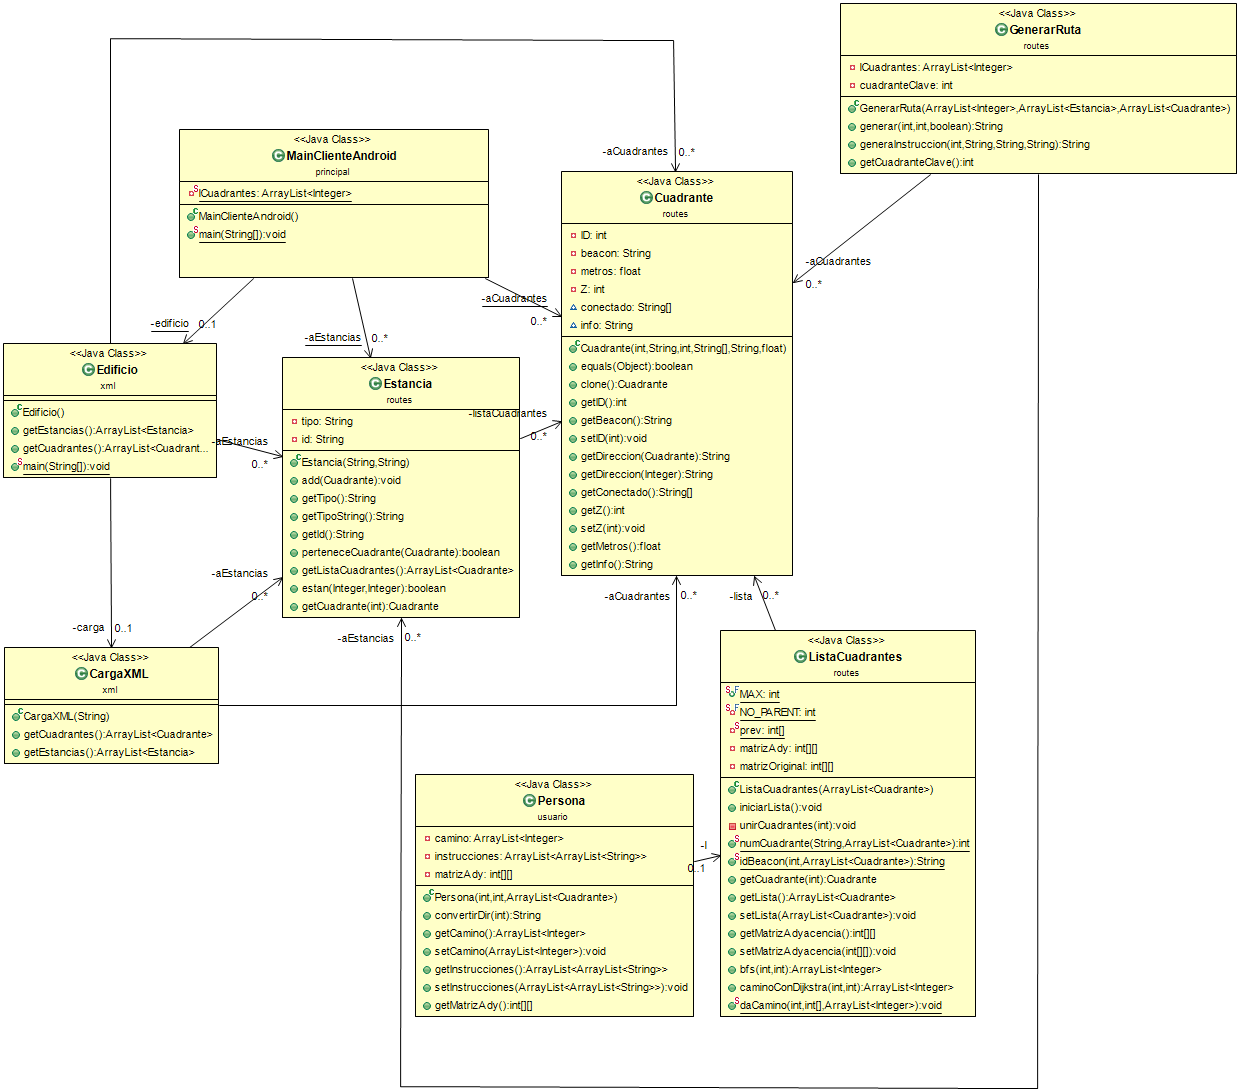
\includegraphics[width=1.1\textwidth]{Imagenes/Capitulo4/diagramServer}
	\caption{Diagrama de las clases principales del servidor.}
	\label{fig:diagServ}
\end{figure}




\subsection{Detalles técnicos del posicionamiento}

A diferencia de todos los trabajos previos de guía que se han hecho en la Facultad de Informática (comenzando por AVANTI, PONER REFERENCIA), el nuestro introduce una tecnología nueva y en pleno auge: los ya conocidos \textit{beacons}. Esto supone un gran cambio en el sistema de posicionamiento, ya que eliminamos por completo la triangulación y nuestro servidor recibe información solo del beacon más próximo al cliente. En función de ese dato, determina el cuadrante en el que se encuentra y qué movimientos debe hacer el usuario.  Veamos, de manera general, el funcionamiento del servidor cada vez que llega un nuevo cliente:

\begin{enumerate}
	\item El servidor recibe el beacon más cercano que tiene el cliente y el destino al que quiere ir. En base a eso reconoce los cuadrantes origen y destino.
	
	\item Calcula la ruta óptima (en lo que sigue veremos a qué nos referimos con esto) que debe seguir el cliente desde el origen o posición actual del cliente para llegar al destino. 
\end{enumerate}

El cliente va llamando al servidor cuando actualiza su posición actual, de esta manera el servidor puede ir actualizando también las instrucciones. Una vez que la ruta ha finalizado, el servidor se lo indica al cliente con una instrucción de finalización. Por ejemplo, \textit{su destino se encuentra a la derecha, el recorrido ha finalizado}.

\subsection{Cálculo de la ruta óptima e instrucciones de guía}
\label{rutaEInst}

Una vez que el mapeo del edificio y el posicionamiento del usuario están resueltos es hora de comenzar a trabajar en la guía. El mapeo que hemos visto en la Sección \ref{sec:mapeo}, ya nos proporciona un grafo, pues pasar de los cuadrantes a esta estructura de grafo es algo relativamente fácil con el uso de una matriz de adyacencia. De esta manera, el cálculo de la ruta más corta entre dos cuadrantes se reduce a uno de los tantos problemas similares que hemos visto durante nuestros años en la Facultad. Es claro que el algoritmo de \textit{Dijkstra} supone la solución al problema, y así lo implementamos.

Sin embargo, no debemos olvidar que nuestra aplicación tiene un usuario final muy concreto: las personas con discapacidad visual. Es por ello que la ruta debía ser la más fácil para ellos, no la más corta necesariamente. Nos dimos cuenta al hacer pruebas de distintas rutas, concretamente una que salía desde la puerta principal de la facultad y terminaba en la puerta trasera de la cafetería: el algoritmo de \textit{Dijkstra} nos sugirió que el camino más corto era pasando por detrás de conserjería (ver cuadrante 32 en PONER REFERENCIA DE LA FOTO DE LOS CUADRANTES) y no se equivocaba, es la ruta más corta en cuanto a cuadrantes pero no la óptima para una persona con discapacidad visual, pues ese pasillo es más estrecho y la gente se suele aglomerar, (están los ascensores, la gente continúa su camino a la cafetería o a la calle por ahí, etc) además de que el usuario tiene que hacer más giros. Mucho más conveniente sería continuar la ruta por delante de Secretaría y luego girar a la izquierda. Para lograrlo, simplemente añadimos más peso en nuestra matriz de adyacencia a aquellas conexiones que creímos más complicadas, en este caso a las conexiones entre los cuadrantes 31-32 y 32-22. De esta manera hacemos que el paso por el pasillo de los ascensores se limite únicamente al caso en el es estrictamente necesario pasar por allí, es decir, cuando se necesitan los ascensores.